%\documentclass[11pt]{amsart}
\documentclass[review]{siamart}
\usepackage{geometry}                % See geometry.pdf to learn the layout options. There are lots.
\geometry{letterpaper}                   % ... or a4paper or a5paper or ... 
%\geometry{landscape}                % Activate for for rotated page geometry
%\usepackage[parfill]{parskip}    % Activate to begin paragraphs with an empty line rather than an indent
\usepackage{graphicx}
\usepackage{amssymb}
\usepackage{epstopdf}
%\usepackage{color}

\DeclareGraphicsRule{.tif}{png}{.png}{`convert #1 `dirname #1`/`basename #1 .tif`.png}
\newcommand{\Order}[1]{\ensuremath{\mathcal{O}(#1)}}    % big O notation


\title{Algorithms and software for extreme-scale solvers in XGC}
\author{Mark F. Adams\and Mathew Knepley\and Tobin Issac}
\nolinenumbers
\begin{document}
\maketitle

{\centering
  \$150,000 per year\par}
\vskip .5cm 

Simulating highly magnetized fusion plasmas, with the discretization and model accuracy necessary to be relevant to ITER's design and operation, is one of the great computational science challenges of today and is of significant programmatic  importance to the DOE.
XGC is the DOE's flagship code for full plasma modeling and it has the potential for engineering relevance to ITER \cite{Chang09}.
While the mesh, discretization, and equation solver methods, the ``solvers" herein, in XGC have been effective for over a decade, the newer numerical methods, such as implicit time integrators, are placing higher demands on accuracy and robustness.
For instance, some of these methods require 3D solvers, which are much more demanding than the current 2D finite element Poisson solvers on fairly isotropic grids.
XGC currently uses highly stretched grids, required to reduce the memory footprint because the full grid data is replicated in each address space.
Stretched grids are not accurate and are difficult to solve efficiently with iterative equation solvers, i.e., algebraic multigrid (AMG).
XGC uses low order accurate discretizations, finite differencing in the parallel direction and finite elements in the perpendicular plane.
These low order discretizations, combined with memory constraints, limit the accuracy of the XGC solvers.
Additionally, the challenges of emerging architectures are changing the balance of costs from flops to memory movement, which does not favor AMG methods because they have low arithmetic intensity.

We propose to address these challenges by redesigning the solver algorithms and data partitioning and algorithms (data models) for XGC.
There are several facets to this proposal.
The key observation that motivates our design is that while AMG methods are very successful, and will continue to be widely use for the foreseeable future because of their ease of interfacing with application codes, they are not well suited to emerging architectures and they are in fact mathematically weaker than classical geometric multigrid (GMG) methods \cite{Brandt-77}.
GMG is not widely because it is difficult to deploy flexible and efficient GMG equation solvers in a library, to amortize their cost of development, because they are inherently tied to the meshing and discretizations.
We at PETSc believe we have a solution to this deployment problem.
First, modern grid and adaptive mesh refinement (AMR) discretization methods have been developed in the p4est distributed tree library \cite{DBLP:journals/siamsc/IsaacBWG15,Rudi:2015:EIS:2807591.2807675,Stadler1033}, and are being added to PETSc in our Solver Integrated Tree-based Adaptive Refinement (SITAR) infrastructure in the DMPICell object.
Second, modern commercial grade software engineering practices and mesh abstraction layers in PETSc make the relatively tight coupling with applications practical for high value applications, if not for the masses of PETSc users \cite{KnepleyBrownMcInnesSmithRuppAdams2015b}.
We propose to continue, and accelerate, the development PICell solvers specialized for the particular demands of extremes scale anisotropic PIC methods in general and XGC in particular.

\section{Budget and Milestones}
\label{sec:mile}

%This section lists the capabilities that need to be added to PETSc and X2 to first understand, drive, and verify the algorithms and implementations in PETSc, and second to build up the capabilities in X2 to be potentially useful for some physics campaigns for which very accurate and scalable solvers are necessary. 
This work leverages projects in the ASCR base program, the DOE FASTMath institute, and an Intel Parallel Processing Center (IPPC), which funds Dr. Tobin Issac.
The work propose here takes place in the PETSc library and a tokamak PIC code, X2 (\S\ref{sec:x2}), to develop data models, verify, and otherwise drive, the PETSc development.
Professor Matthew Knepley at Rice University (\$75,000 per year) and his student will work on the PETSc development and Dr. Mark Adams (\$75,000 per year) will work with Professors Christlieb and Verboncoeur at Michigan State University, East Lansing, and a plasma science student, on the X2 work.
The following tasks are proposed for this project by Professor Knepley's team [K] and Dr. Adams' team [A], with the quarter of completion unless otherwise stated.
\vskip .1cm 
\begin{itemize}
\item Complete core PIC functionality in DMPICell and add to X2 [A,K: FY16 Q3]:
\begin{enumerate}
\item Point location in grid (done for flux tubes)
\item Point gradient (cell to particle methods)
\item Point deposition (particle to cell method)
\item Poisson solver with non-constant material coefficients 
\end{enumerate}
\item Optimize a kernel (e.g., deposition) for KNL with IPCC to better understand primary performance issues [A: FY16 Q4]
\begin{itemize}
\item Similarly optimize kernel for GPUs depending on resources and interest
\end{itemize}
\item Add adiabatic electron, electrostatic, gyrokinetic capability [A: FY17 Q2]
\begin{itemize}
\item Begin investigating accuracy requirements in grid methods (e.g., gradients) 
\end{itemize}
\item Add $B_0$ point interpolation [A: FY17 Q2]
\item Add ghost cells and particle deposition communication, as needed, for gyrokinetics, and begin optimizing data models [A,K: FY17 Q2]
\item Q2 elements [K: FY17 Q2]
\item Begin to develop performance models with physics to prepare for particular exa-scale physics campaigns [A,K: FY17 Q2]
\item Improve visualization with combined particles and grid [A: FY17 Q3]
\item Finite particle form factors or density smoothing [A: FY17 Q4]
\end{itemize}
\vskip .1cm 
We intend to seek funding for a second year for the following work.
\vskip .1cm 
\begin{itemize}
\item Begin convergence studies for verification on model problem (e.g., Cyclone benchmark with adiabatic electrons and electro-statics) [A: FY18 Q1]
\item Begin code to code verification with XGC1 [A: FY18 Q2]
\item Continue adding physics, verifying accuracy, optimizing code, and optimizing data models [A,K: FY18 Q4]
%\item Work with RPI team in evaluating data models and performance models [FY18]
\end{itemize}
%\pagebreak

\section{Introduction}

The high degree of concurrency of emerging architectures at extreme-scale, and the high relative cost of data movement, requires careful data placement for optimal performance.
The importance of data locality is not new, the pressures on memory systems have been building for decades because floating point processing speeds increase faster than data movement speeds, but the massive concurrency of emerging architectures is further exacerbating the need for careful data layout in extreme-scale computing.
This is a challenge for PIC codes because they process data in two very different data structures, which interact in particle-cell kernels such as charge deposition to the grid and particle gradient computation from the grid.
Additionally, optimal data decompositions of different computational components can be very different.
For instance, the collision operator in XGC and the deposit, solve, push phase have inherently different natural data partitionings, and a ``transpose" to move particle between these partitions has a cost.
Balancing this cost with the rest of the computation is a common tradeoff in computational science and can be seen in, for instance, the Eulerian fusion plasma code GYSELA \cite{Bigot13}.

The PETSc community has extensive experience in extreme-scale solution methods for PDEs (discretizations, meshing, nonlinear solvers, time integrators, optimization solvers, etc.) and in the deployment of optimized implementations of these methods to the public.
Fast solvers also require careful data placement for optimal performance, but PIC methods add new sets of constraints and opportunities for optimizing algorithms for extreme-scale emerging architectures.
To this end, we focus on grid management to support the development of optimal data decomposition and algorithms, or data models,  for the efficient processing of particle-cell interactions, as well as fast solvers for, for example, Poisson's equation, Ampere's law, and the magnetohydrodymaic  solvers of implicit PIC methods \cite{DBLP:journals/cphysics/ChenC15,Adams-10a}.

We propose to support extreme-scale PIC simulations on emerging architectures in PETS to enable XGC to continue its preeminence for decades to come.
%We build on the Solver Integrated Tree-based Adaptive Refinement (SITAR) infrastructure in PETSc, for fast and accurate PDE discretizations, meshing, and solvers.
%We extend SITAR with methods and features to support the development of efficient and scalable data models and algorithms for engineering relevant simulations of fusion plasmas by the computational plasma physics community.
In addition to this PETSc library work, this document describes a tokamak PIC code, X2 (\S\ref{sec:x2}).
X2 is designed from the ground up for extreme scalability and extensibility to emerging architectures and is modeled on the particle methods in XGC.
X2 is used to drive the library development and explore the algorithmic space of modern extreme scale PIC methods, and to provide data on the potential usefulness of these PETSc resources for XGC.

\section{Background}

PIC methods are popular for discretizing high dimensional problems because of their low cost relative to full grid or Eulerian methods on such problems, although Eulerian methods are often at least hybridized with PIC in, for instance, the collision operator in XGC.
PIC methods do have disadvantages, including more complex data algorithms because of its two distinct data types, particles and cells.
PIC algorithms require three types of processing: 1) particle processing (e.g., the evolution of Vlasov's equation), 2) grid processing (e.g., solvers), and 3) particle-grid interactions (e.g., particle charge deposition and gradients of potentials for particle pushing).
Pure particle processing, such as the ``push" of particles use relatively simple arrays and each particle can be processed concurrently.
Most, say well over $99\%$, of the data in a fusion PIC simulation is in the particles.
Thus, pure grid work, such as the Poisson solver, have abundant computational resources available and, for instance, can be run entirely on the CPU of accelerated architectures, or on a reduced set of cores on symmetric systems.
Particle-grid interactions are challenging because the data structures and natural data decompositions are different, but are tightly coupled algorithmically.
This tight coupling, and the ever-increasing importance of data locality generally, make the data model critical in the current and future extreme-scale PIC applications.

The critical importance of data placement for the efficient processing of PIC methods requires that highly optimal, and potentially complex, data models be developed.
One can avoid much of this code complexity by replicating grid data on each MPI process or address space.
This approach does simplify the data model considerably, however it also removes the most fundamentally important optimization opportunity for extreme-scale PIC codes on emerging architectures.
Distributing grids will be very disruptive to the code base of fusion PIC applications, but many of the optimizations in the context of replicated data will not be applicable, or necessary, on distributed grids \cite{Adams-07a}.
%It behooves the fusion PIC community to move to distributed data models early to begin their optimization.

The physics community has developed a large body of research and experience in using PIC methods for fusion plasmas and they are one of the largest users in DOE leadership class compute facilities.
The applied math, engineering, and physics communities have developed powerful discretization and solver methods for extreme-scale computing in just the past ten years and stretching back to the 1960s, but these modern methods are not widely used in the fusion PIC community.
The continued advancement of computational fusion physics in XGC, and the global community, especially as we move to simulations relevant to the design and operation of ITER, will benefit from both modern numerical methods and parallel computing techniques, and commercial grade software engineering methodologies.

The engineering complexity required to develop a flexible infrastructure that allows for the expression of the most optimal algorithms demands a higher level of software quality assurance processes than is often present in the codes that are driven by academic reward systems, such as number of journal publications, as opposed to the demands for reliable predictive analysis that drives the commercial sector.
Commercial grad software engineering takes both skill and time that is not available to most academic physics code projects and is not seen as worth to cost due to their academic reward structure.
PETSc employs commercial grade software engineering processes and some of our users, even those that work in academia, follow our practices because in the long term it leads to higher productivity even by the standards of their academic field. 
This project provides fusion PIC codes with solid infrastructure on which to build their physics, to allow for the full use of their theoretical expertise without the demands of implementing, verifying, and maintaining the increasing software stack required to effectively use modern hardware.

This work amortizes both the development costs and the intellectual resources required to develop and deploy support for extreme-scale PIC applications.
This work builds on the SITAR framework in PETSc, which provides both fast solvers, tightly integrated meshing and discretizations, and optimized implementation for emerging architectures \cite{KnepleyBrownMcInnesSmithRuppAdams2015}.
SITAR is built on the highly scalable algorithms and implementations in the {\tt p4est} distributed tree library \cite{DBLP:journals/siamsc/IsaacBWG15,Rudi:2015:EIS:2807591.2807675,Stadler1033}.

\section{Methodology}

The methods developed in this project are guided by several general principles in terms of algorithms pursued in X2 and supported in PETSc.
These principles reflect our view of algorithms for extreme-scale fusion PIC methods.
Our methodology has the following desired features:
\begin{itemize}
\item flexible local grids to allow for particle-grid interaction with non-local parts of the grid;
\item hierarchical grids for fast geometric multigrid solvers, AMR, and the ``particle search" method to determine the address space of a particle;
\item grids abstracted from application scientists to allow multiple types of grids and discretizations to be supported and selected at run time;
\item fast linear and nonlinear solvers for Poisson and Ampere's law solvers, and implicit PIC methods (magnetohydrodymaic);
\item incremental problem development for debugging and verification on Cartesian grids and ramping up to full tokamak wall geometries;
\item finite particle form factors, or density smoothing, to allow for arbitrary mesh resolution without increasing particle count to avoid particle noise;
\begin{itemize}
\item allows decoupling grid spacing from the particle form factor and facilitates AMR and convergence test verification;
\end{itemize}
\item finite volume (FV), discontinuous Galerkin(DG), and finite element (FE) discretizations;
\begin{itemize}
\item conservative discretizations (FV and DG) are useful for flux surface averaging projections although we are beginning with FE;
\end{itemize}
\item architecture specific computational kernels for emerging architectures \cite{KnepleyBrownMcInnesSmithRuppAdams2015};
\item incremental contributions to the plasma physics community (\S\ref{sec:id}).
\end{itemize}

\subsection{Incremental Development}
\label{sec:id}

The realization of an engineering relevant full plasma simulation of ITER is a significant multi-year undertaking.
The development plans for this project are to be both incrementally relevant and engaged with the physics community in XGC.
To this end, early deliverables are important, to encourage physicists to participate with us and for us to stay grounded in engineering demands.
To this end we see several early areas that our project can contribute to the XGC project:
\begin{itemize}
\item Distributed data model exploration. Explore data decompositions and collect performance data to help further refine effective distributed data models for fusion PIC applications;
\item Code verification. Cross code verification of existing fusion PIC codes, on somewhat simple model problems, but with full ITER wall geometries;
\item Performance Verification.  Develop performance models of idioms in PIC codes (e.g., equation solvers, particle communications, particle pushing) to help application scientist verify that codes are performing correctly, by understanding the relative costs of different processes and their sensitivities (derivatives with respect to) machine metrics.
\end{itemize}
 

\section{Current and Future Development}
\label{sec:x2}

The development proposed herein takes place in a branch in the PETSc repository (mark/feature-picell) and a driver application named X2 (DMPICell ex1.c).
Code will likely migrate from X2 into the PETSc library as development progresses.
X2 is used to gather initial performance data on modern architectures to guide further data model developments, and to verify the PETSc library code.
Our approach is to exploit the fact that particle distributions, at least from a computational point of view, are relatively uniformly distributed over the domain.
This allows for particle distributions that are simply attached to cells of the solver grid, but load is balanced by using a weighted cell partitioning because we use unstructured AMR.
Note, SITAR supports tree-based AMR in addition to unstructured AMR, but we plan on using uniform refinement for the foreseeable future.

We currently use guide center particles only (i.e., only a parallel velocity, resulting in a 4D method), which simplifies charge deposition.
This allow us to reuse particle infrastructure that has been developed for other PETSc PIC users \cite{may2014ptatin} that attach particle to solver cells in the particle push kernel.
More complex data models with extended halo regions to accommodate gyrokinetic methods (finite shape) and high order time integrators will likely be required in the future.

The collision operator is a computational intensive nonlinear solve in velocity space on each particle collision cell.
Flux tubes are a natural choice for these collision cells.
Flux tubes are long, narrow subdomains that follow the twisting magnetic field lines in a tokamak.
We decouple the grid partitioning from the flux tube partitioning and implement a full ``transpose" of particles between these two partitions.
Aligning the solver partitioning with flux tubes, to minimize communication, is a probable future optimization.

Figure \ref{fig:cross} (left) shows half of a 64 a flux tube particle mesh; Figure \ref{fig:cross} (right) shows an example of an ITER grid.
\begin{figure}[h!]
   \centering
   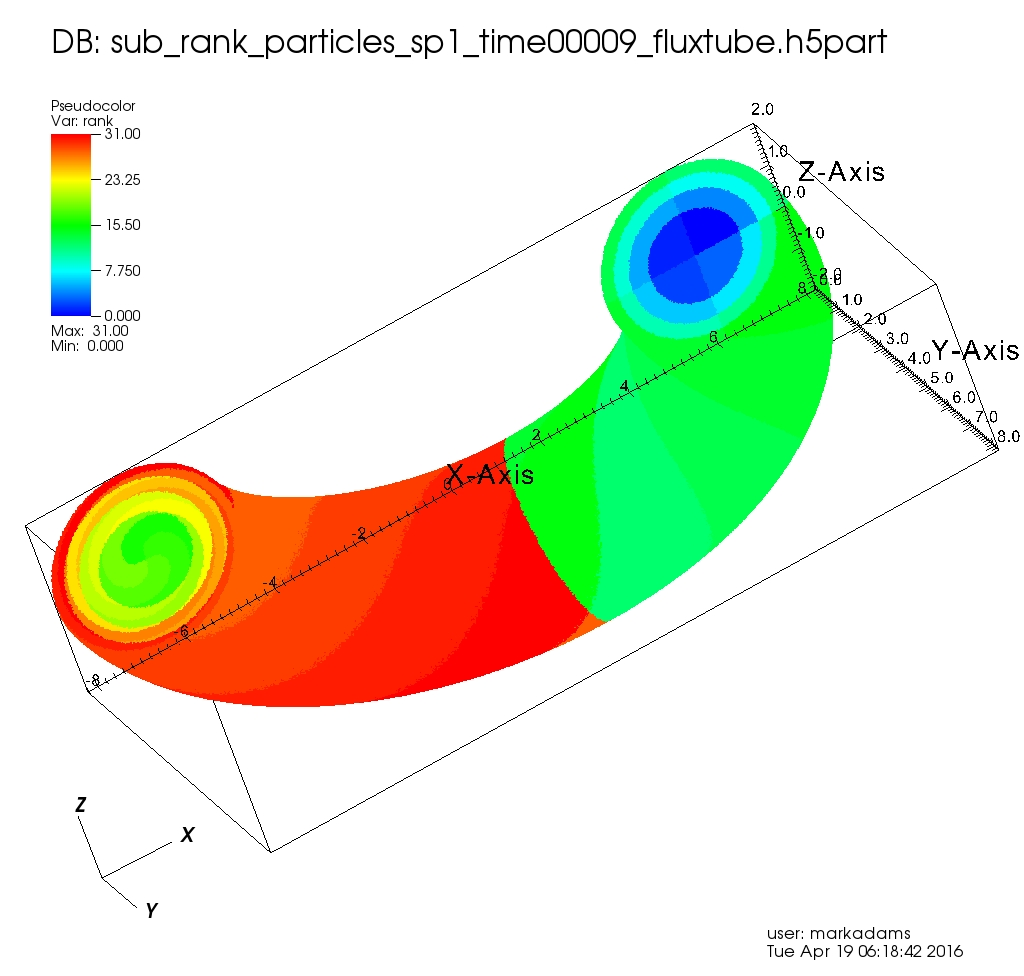
\includegraphics[width=70mm]{half_fluxtubes_64.jpeg} 
    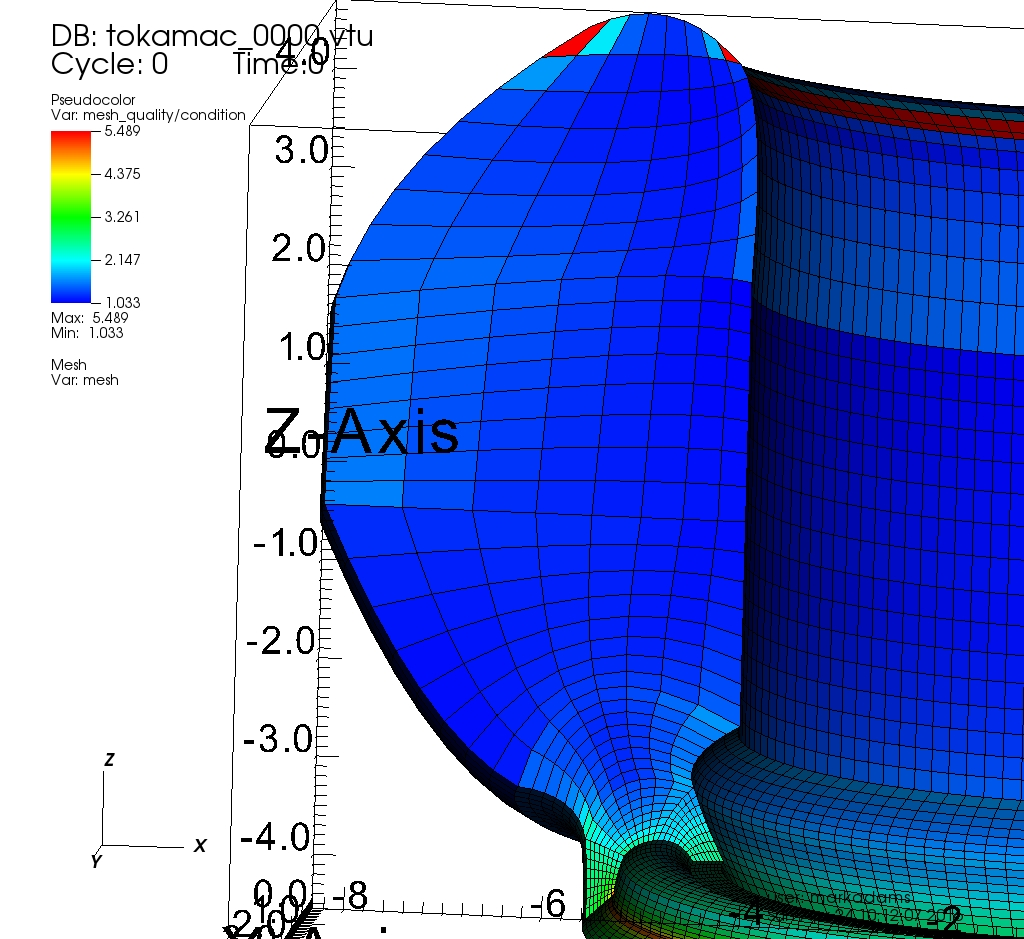
\includegraphics[width=80mm]{half_half_grid_mesh.jpeg} 
   \caption{Half of  2x2x2 flux tube particle partition of torus (left), corresponding coarse ITER grid solver mesh (right), colored by condition number of the elements}
   \label{fig:cross}
\end{figure}
The fuzzy edges of Figure \ref{fig:cross} (left) are due to the finite number of particles, each particle is colored with the rank of the partition to which it belongs.

X2's design principles are modeled on those of PETSc, in terms of extensibility and flexibility.
The X2 kernels are mesh independent, which allows the meshes to be selected at run time.
This allows us to incrementally develop and verify new capabilities on simpler problems before moving to more realistic geometries.
This is critical in continuously verify the code and an effective develop, debug, and verify code cycle.
To this end we currently support Cartesian grids  (e.g., Figure \ref{fig:grids}, left) and circular cross section toruses (e.g., Figure \ref{fig:grids}, right).
\begin{figure}[h!]
   \centering
   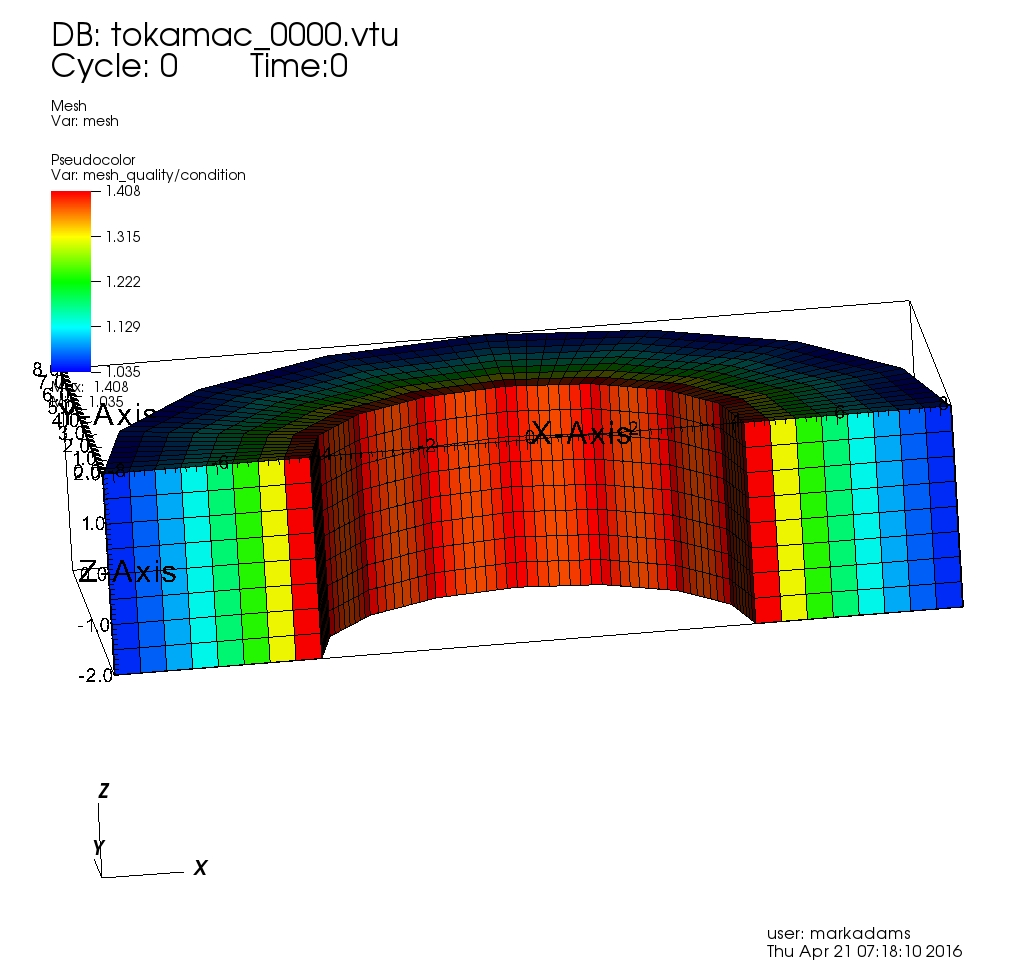
\includegraphics[width=70mm]{half_box_torus.jpeg} 
    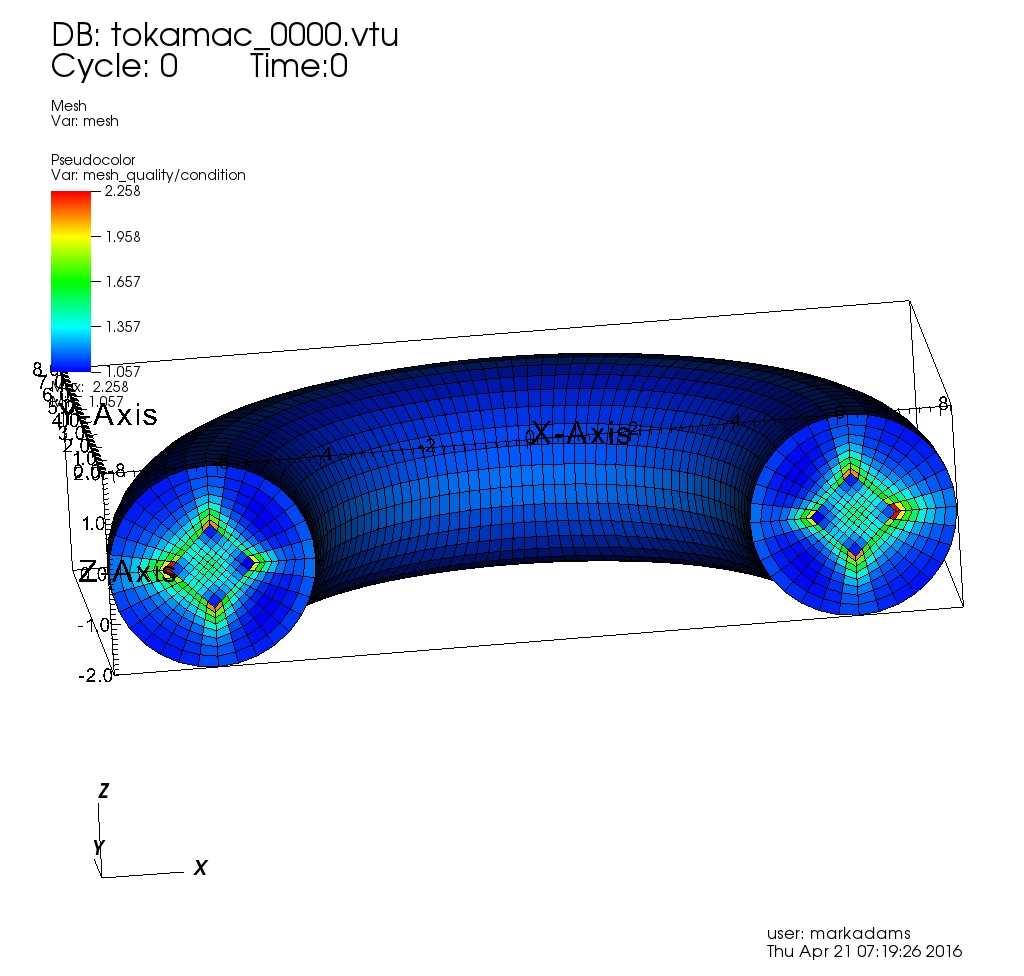
\includegraphics[width=80mm]{half_torus.jpeg} 
   \caption{Half of a Cartesian cross section torus (left), and circular cross section tokamak (right), colored by condition number of the elements}
   \label{fig:grids}
\end{figure}

\subsection{High Order}
\label{sec:ho}

The mesh in Figure \ref{fig:cross} (right) is generated with seven (high order) Q2 elements per plane on a coarse grid and is refined three times in this figure.
%We currently use trilinear elements, which results in 28 elements per plane on the coarse grid.
High order elements are attractive because of their high accuracy for smooth solutions should allow for fewer vertices and hence larger ``cells".
Furthermore, because order elements are in effect composed of multiple cells they are even larger in physical space.
Large elements are useful because we build the particle data structure around them, larger elements results in larger element particle lists, which is beneficial for vectorization.
Additionally, the solutions of say the Poisson solve in fusion applications, with turbulence, are smooth at the scale of the (known) Larmore radius and, in fact, physicists often smooth the results of low order Poisson solvers to reduce high frequency components.
Q2 elements can also capture curved surface better than linear elements (Figure \ref{fig:cross}, right).
We plan to move to discontinuous Galerkin (DG) methods in the future because they have attractive mathematical properties, such as having rigorous theory like finite elements and being conservative like finite volume, which would be useful for flux surface averaging projections.
%DG results in systems with many degrees of freedom, a common problem of these methods, but fusion PIC solvers are highly over provisioned with processing resources, thus, local work and storage complexity are not critical for these solves.

\bibliographystyle{siamplain}
\bibliography{./bib} 
\end{document}  